\documentclass[t,pdf]{beamer}
\mode<presentation>{}


\usecolortheme[RGB={196, 30, 58}]{structure}
\definecolor{lightgreen}{RGB}{ 220, 255, 220}
\definecolor{lightblue}{RGB}{ 220, 220, 255}

\usepackage{color}
\usepackage{animate}
\usepackage{tikz}
\usetikzlibrary{shadings,shadows}
\usetikzlibrary{shapes, arrows}
\usetikzlibrary{decorations.pathreplacing,angles,quotes}
\usetikzlibrary{calc}
\usetikzlibrary{positioning}
\usepackage{pgfplots}
\usepackage{booktabs,colortbl}
\usepackage{graphicx}

\usepackage{alltt}
\newenvironment{ccode}{\begin{alltt}\footnotesize}{\end{alltt}}


\usepackage{hyperref}
%% Colored hyperlink 
\newcommand{\cref}[2]{\href{#1}{\color{blue}#2}}
%% Colored hyperlink showing link in TT font
% \newcommand{\chref}[1]{\href{#1}{\small\tt \color{blue}#1}}
\newcommand{\hcref}[1]{\cref{#1}{\small\tt #1}}

\usepackage{booktabs,colortbl}

\newcommand{\keyword}[1]{\textbf{#1}}
\newcommand{\keyif}{\keyword{if}}
\newcommand{\keywhile}{\keyword{while}}
\newcommand{\keyfor}{\keyword{for}}
\newcommand{\keytrue}{\keyword{True}}
\newcommand{\keybreak}{\keyword{break}}
\newcommand{\keyreturn}{\keyword{return}}
\newcommand{\assign}{\ensuremath{\longleftarrow}}



\newcommand{\ground}{blue}
\definecolor{xred}{rgb}{0.77, 0.12, 0.23}
\definecolor{xgreen}{rgb}{0.3, 0.6, 0}
\definecolor{xblue}{rgb}{0., 0.25, 1}
\tikzstyle{grayfill} = [fill=fillcolor!70, draw=drawcolor, thick]
\tikzstyle{whitefill} = [fill=white, draw=drawcolor, thick] 
\definecolor{fillcolor}{rgb}{0.5, 0.5, 0.5} 
\definecolor{drawcolor}{rgb}{0, 0, 0} 

\definecolor{medgreen}{rgb}{0.34, 0.65, 0.34}
\definecolor{clearorange}{rgb}{0.917647, 0.462745, 0}
\definecolor{darkred}{rgb}{0.576471, 0.152941, 0.172549}


\definecolor{mediumgreen}{RGB}{20,140,20}
\definecolor{mediumblue}{RGB}{20,20,140}

\definecolor{bddneutralcolor}{RGB}{0,0,102}
\definecolor{bddpathcolor}{RGB}{25,25,255}
\definecolor{bddfillcolor}{RGB}{255,255,224}
\definecolor{bddbackground}{RGB}{230,240,255}
\definecolor{bddhighcolor}{RGB}{204,0,0}
\definecolor{bddlowcolor}{RGB}{0,143,0}



\definecolor{xred}{rgb}{0.77, 0.12, 0.23}
\definecolor{xgreen}{rgb}{0.3, 0.6, 0}
\definecolor{xblue}{rgb}{0., 0.25, 1}
\tikzstyle{grayfill} = [fill=fillcolor!70, draw=drawcolor, thick]
\tikzstyle{whitefill} = [fill=white, draw=drawcolor, thick] 
\definecolor{fillcolor}{rgb}{0.5, 0.5, 0.5} 
\definecolor{drawcolor}{rgb}{0, 0, 0} 

\title{Trustworthy Boolean Reasoning \\ 2B: Proof Generation with BDDs}
%\subtitle{}
\author{Randal E. Bryant}


\institute{
\includegraphics[height=50pt]{figs/CMU_Logo}}

\date{\textcolor{black}{June, 2022}}

\setbeamertemplate{footline}
{
	\leavevmode%
	\hbox{%
	\begin{beamercolorbox}[wd=0.35\paperwidth,ht=2.25ex,dp=1ex,center]{author in head/foot}%
	\tiny {Bryant: SSFT22}
			\vspace{4pt}
	\end{beamercolorbox}%
	\begin{beamercolorbox}[wd=0.45\paperwidth,ht=2.25ex,dp=1ex,center]{author in head/foot}%
	\end{beamercolorbox}%
	\begin{beamercolorbox}[wd=0.2\paperwidth,ht=2.5ex,dp=1ex,right]{date in head/foot}%
		\structure{\scriptsize \insertframenumber{} / \inserttotalframenumber\hspace*{3ex}}
		\vspace{3pt}
	\end{beamercolorbox}}%
	\vskip0pt%
}

\beamertemplatenavigationsymbolsempty

\begin{document}

\newcommand{\R}{\mathbb{R}}
\renewcommand{\P}{\mathbb{P}}
\newcommand{\E}{\mathbb{E}}
\newcommand{\Z}{\mathbb{Z}}
\newcommand{\N}{\mathbb{N}}
\newcommand{\diam}{\mbox{diam}}

\newcommand{\obar}[1]{\overline{#1}}
\newcommand{\anot}{\obar{a}}
\newcommand{\bnot}{\obar{b}}
\newcommand{\cnot}{\obar{c}}
\newcommand{\dnot}{\obar{d}}
\newcommand{\tnot}{\obar{t}}
\newcommand{\unot}{\obar{u}}
\newcommand{\vnot}{\obar{v}}
\newcommand{\wnot}{\obar{w}}
\newcommand{\xnot}{\obar{x}}
\newcommand{\znot}{\obar{z}}
\newcommand{\ite}{{\it ITE}}

\newcommand{\btrue}{1}
\newcommand{\bfalse}{0}

\newtheorem{conjecture}[theorem]{Conjecture}
\newtheorem{nonconj}[theorem]{(Not actually a) conjecture}


\AtBeginSection[]{
\begin{frame}{Table of Contents}
	\tableofcontents[currentsection]
\end{frame}
}

\begin{frame}
	\titlepage
\end{frame}

\frame{
  \frametitle{Important Ideas for These Lectures}
  \begin{itemize}
  \item SAT solvers are useful tools
    \begin{itemize}
    \item Many practical problems reducible to SAT
    \item Need to learn effective encoding techniques
    \end{itemize}
\medskip
  \item For many applications, formulas should be unsatisfiable
    \begin{itemize}
    \item Program should generate a checkable proof
    \item There is a well-developed proof infrastructure
    \end{itemize}

\medskip
  \item {\bf Binary Decision Diagrams (BDDs) can play important role}
    \begin{itemize}
    \item In supplementing current SAT algorithms
    \item {\bf In proof generation}
    \end{itemize}
  \end{itemize}
}





\begin{frame}
  \frametitle{Extended Resolution and BDDs}
  
\begin{itemize}
\item Tseitin, 1967
\end{itemize}

{\bf Can introduce extension variables}
\begin{itemize}
\item Variable $z$ that has not yet occurred in proof
\item Must add {\em defining} clauses
\begin{itemize}
\item Encode constraint of form $z \leftrightarrow F$
\item Boolean formula $z$ over input and earlier extension variables
\end{itemize}
\end{itemize}

\medskip

{\bf Extension variable $z$ becomes shorthand for formula $F$}
  \begin{itemize}
  \item Repeated use can yield exponentially smaller proof
  \end{itemize}

  \medskip
\only<2->{
      {\bf Generate extension variable for every node in BDD}
      \begin{itemize}
        \item Biere, Sinz, Jussila, 2006
        \item Each recursive step of Apply algorithm justified as proof steps
        \item Reducing formula to BDD $\bot$ yields UNSAT proof
      \end{itemize}
}
\end{frame}

\frame{
\frametitle{Generating Extended Resolution Proofs}

\begin{itemize}
\item Create extension variable for each node in BDD
\begin{itemize}
\item Notation: Same symbol for node and its extension variable
\end{itemize}
\end{itemize}

\begin{center}
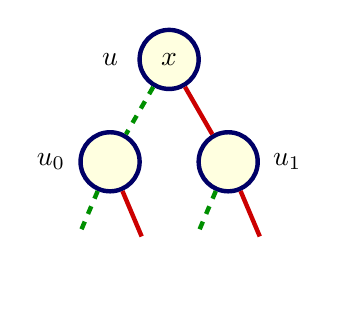
\begin{tikzpicture}
\node[circle,ultra thick,fill=bddfillcolor,draw=bddneutralcolor,draw,minimum size=0.75cm] (x) at (0,0) {$x$};
\node (u) at (-0.75,0) {$u$};
\node[circle,ultra thick,fill=bddfillcolor,draw=bddneutralcolor,draw,minimum size=0.75cm] (l) at (-0.75,-1.3) {$~$};
\node (u1) at (-1.5,-1.3) {$u_0$};
\node[circle,ultra thick,fill=bddfillcolor,draw=bddneutralcolor,draw,minimum size=0.75cm] (r) at (.75,-1.3) {$~$};
\node (u2) at (1.5,-1.3) {$u_1$};
\node[circle,minimum size=0.75cm] (ll) at (-1.3,-2.6) {$~$};
\node[circle,minimum size=0.75cm] (lr) at (-.2,-2.6) {$~$};
\node[circle,minimum size=0.75cm] (rl) at (.2,-2.6) {$~$};
\node[circle,minimum size=0.75cm] (rr) at (1.3,-2.6) {$~$};
\draw[ultra thick, color=bddlowcolor,dashed] (x) -- (l);
\draw[ultra thick, color=bddhighcolor] (x) -- (r);
\draw[ultra thick, color=bddlowcolor,dashed] (l) -- (ll);
\draw[ultra thick, color=bddhighcolor] (r) -- (rr);
\draw[ultra thick, color=bddlowcolor,dashed] (r) -- (rl);
\draw[ultra thick, color=bddhighcolor] (l) -- (lr);
\end{tikzpicture}
\end{center}

\vspace{-25pt}

\begin{itemize}
\item Defining clauses encode constraint $u \leftrightarrow {\sf ITE}(x, u_1, u_0)$
\end{itemize}
\medskip

\centering

\begin{tabular}{ccc}
\rowcolor{structure}\textcolor{white}{Clause name} & \textcolor{white}{~~~Formula~~~} & 
\textcolor{white}{~~Clausal form~~} \\[3pt]
\rowcolor{xgreen!20!white} ${\sf HD}(u)$ & $x \rightarrow (u \rightarrow u_1)$ & $\xnot \lor \unot \lor u_1$\\
\rowcolor{xgreen!30!white}${\sf LD}(u)$ & $\xnot \rightarrow (u \rightarrow u_0)$ & $x \lor \unot \lor u_0$\\
\rowcolor{xgreen!20!white}${\sf HU}(u)$ & $x \rightarrow (u_1 \rightarrow u)$ & $\xnot \lor \unot_1 \lor u$\\
\rowcolor{xgreen!30!white}${\sf LU}(u)$ & $\xnot \rightarrow (u_0 \rightarrow u)$ & $x \lor \unot_0 \lor u$\\
\end{tabular}



}

\frame{
\frametitle{Apply Algorithm Recursion}

\bigskip

\begin{minipage}{.45\textwidth}
\centering
${\sf Apply} (u,v,\land)$\\[10pt]
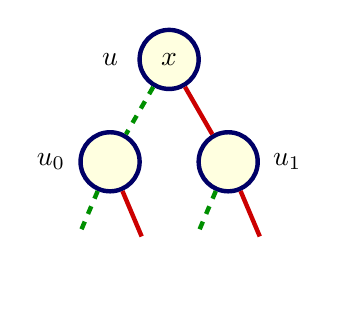
\begin{tikzpicture}
\node[circle,ultra thick,fill=bddfillcolor,draw=bddneutralcolor,minimum size=0.75cm] (x) at (0,0) {$x$};
\node (u) at (-0.75,0) {$u$};
\node[circle,ultra thick,fill=bddfillcolor,draw=bddneutralcolor,draw,minimum size=0.75cm] (l) at (-0.75,-1.3) {$~$};
\node (u1) at (-1.5,-1.3) {$u_0$};
\node[circle,ultra thick,fill=bddfillcolor,draw=bddneutralcolor,draw,minimum size=0.75cm] (r) at (.75,-1.3) {$~$};
\node (u2) at (1.5,-1.3) {$u_1$};
\node[circle,minimum size=0.75cm] (ll) at (-1.3,-2.6) {$~$};
\node[circle,minimum size=0.75cm] (lr) at (-.2,-2.6) {$~$};
\node[circle,minimum size=0.75cm] (rl) at (.2,-2.6) {$~$};
\node[circle,minimum size=0.75cm] (rr) at (1.3,-2.6) {$~$};
\draw[ultra thick, color=bddlowcolor,dashed] (x) -- (l);
\draw[ultra thick, color=bddhighcolor] (x) -- (r);
\draw[ultra thick, color=bddlowcolor,dashed] (l) -- (ll);
\draw[ultra thick, color=bddhighcolor] (r) -- (rr);
\draw[ultra thick, color=bddlowcolor,dashed] (r) -- (rl);
\draw[ultra thick, color=bddhighcolor] (l) -- (lr);
\end{tikzpicture}

\bigskip

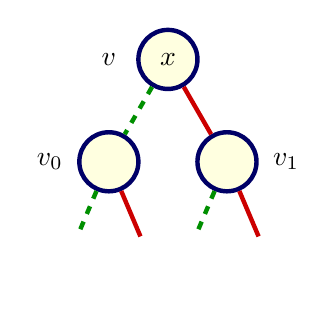
\begin{tikzpicture}
\node[circle,ultra thick,fill=bddfillcolor,draw=bddneutralcolor,draw,minimum size=0.75cm] (x) at (0,0) {$x$};
\node (v) at (-0.75,0) {$v$};
\node[circle,ultra thick,fill=bddfillcolor,draw=bddneutralcolor,draw,minimum size=0.75cm] (l) at (-0.75,-1.3) {$~$};
\node (v1) at (-1.5,-1.3) {$v_0$};
\node[circle,ultra thick,fill=bddfillcolor,draw=bddneutralcolor,draw,minimum size=0.75cm] (r) at (.75,-1.3) {$~$};
\node (v2) at (1.5,-1.3) {$v_1$};
\node[circle,minimum size=0.75cm] (ll) at (-1.3,-2.6) {$~$};
\node[circle,minimum size=0.75cm] (lr) at (-.2,-2.6) {$~$};
\node[circle,minimum size=0.75cm] (rl) at (.2,-2.6) {$~$};
\node[circle,minimum size=0.75cm] (rr) at (1.3,-2.6) {$~$};
\draw[ultra thick, color=bddlowcolor,dashed] (x) -- (l);
\draw[ultra thick, color=bddhighcolor] (x) -- (r);
\draw[ultra thick, color=bddlowcolor,dashed] (l) -- (ll);
\draw[ultra thick, color=bddhighcolor] (r) -- (rr);
\draw[ultra thick, color=bddlowcolor,dashed] (r) -- (rl);
\draw[ultra thick, color=bddhighcolor] (l) -- (lr);
\end{tikzpicture}
\end{minipage}
\hfill
\begin{minipage}{.52\textwidth}
\centering
\pause
Recursion\\[5pt]

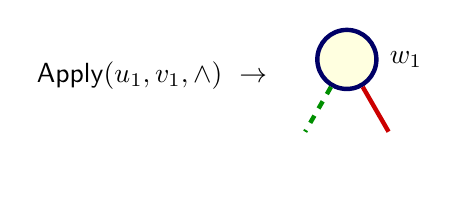
\begin{tikzpicture}
\node at (-2.3,-.2) {${\sf Apply} (u_1,v_1,\land)~\rightarrow~~~$};
\node[circle,ultra thick,fill=bddfillcolor,draw=bddneutralcolor,draw,minimum size=0.75cm] (x) at (0,0) {~};
\node (u) at (0.75,0) {$w_1$};
\node[minimum size=0.75cm] (l) at (-0.75,-1.3) {$~$};
\node[minimum size=0.75cm] (r) at (.75,-1.3) {$~$};
\draw[ultra thick, color=bddlowcolor,dashed] (x) -- (l);
\draw[ultra thick, color=bddhighcolor] (x) -- (r);
\end{tikzpicture}
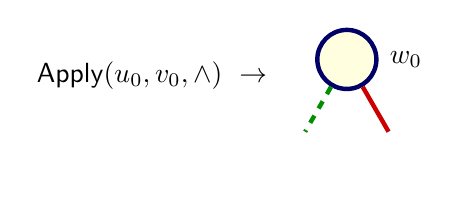
\begin{tikzpicture}
\node at (-2.3,-.2) {${\sf Apply} (u_0,v_0,\land)~\rightarrow~~~$};
\node[circle,ultra thick,fill=bddfillcolor,draw=bddneutralcolor,draw,minimum size=0.75cm] (x) at (0,0) {~};
\node (u) at (0.75,0) {$w_0$};
\node[minimum size=0.75cm] (l) at (-0.75,-1.3) {$~$};
\node[minimum size=0.75cm] (r) at (.75,-1.3) {$~$};
\draw[ultra thick, color=bddlowcolor,dashed] (x) -- (l);
\draw[ultra thick, color=bddhighcolor] (x) -- (r);
\end{tikzpicture}

\vspace{-15pt}
\pause
Result\\[10pt]
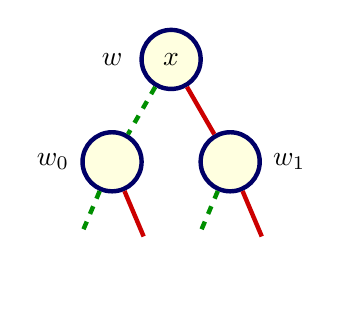
\begin{tikzpicture}
\node[circle,ultra thick,fill=bddfillcolor,draw=bddneutralcolor,draw,minimum size=0.75cm] (x) at (0,0) {$x$};
\node (w) at (-0.75,0) {$w$};
\node[circle,ultra thick,fill=bddfillcolor,draw=bddneutralcolor,draw,minimum size=0.75cm] (l) at (-0.75,-1.3) {$~$};
\node (w1) at (-1.5,-1.3) {$w_0$};
\node[circle,ultra thick,fill=bddfillcolor,draw=bddneutralcolor,draw,minimum size=0.75cm] (r) at (.75,-1.3) {$~$};
\node (w2) at (1.5,-1.3) {$w_1$};
\node[circle,minimum size=0.75cm] (ll) at (-1.3,-2.6) {$~$};
\node[circle,minimum size=0.75cm] (lr) at (-.2,-2.6) {$~$};
\node[circle,minimum size=0.75cm] (rl) at (.2,-2.6) {$~$};
\node[circle,minimum size=0.75cm] (rr) at (1.3,-2.6) {$~$};
\draw[ultra thick, color=bddlowcolor,dashed] (x) -- (l);
\draw[ultra thick, color=bddhighcolor] (x) -- (r);
\draw[ultra thick, color=bddlowcolor,dashed] (l) -- (ll);
\draw[ultra thick, color=bddhighcolor] (r) -- (rr);
\draw[ultra thick, color=bddlowcolor,dashed] (r) -- (rl);
\draw[ultra thick, color=bddhighcolor] (l) -- (lr);
\end{tikzpicture}

\end{minipage}

}

%% \frame{
%% \frametitle{Apply Algorithm Nuances}

%% {\bf Stop recursion when hit terminal case}
%% \begin{itemize}
%% \item $f \land 0	 \rightarrow	 0$ $\qquad\qquad$	$0 \land g 	 \rightarrow	 0$
%% \item $f \land 1	 \rightarrow	 f$ $\qquad\qquad$	$1 \land g 	 \rightarrow	 g$
%% \item $f \land f 	 \rightarrow	 f$
%% \end{itemize}
%% \smallskip

%% {\bf Special cases for recursion}
%% \begin{itemize}
%% \item $u$ and $v$ have different top-level variables
%% \item Recursion returns values with $w_1 = w_0$  
%% \end{itemize}  
%% \smallskip

%% {\bf Operation Cache contains previously computed results}
%% \begin{itemize}
%% \item $[u, v, \land] \rightarrow w$
%% \item Guarantees polynomial performance
%% \end{itemize}
%% \smallskip

%% {\bf Unique Table contains all generated nodes}
%% \begin{itemize}
%% \item $[x, u_1, u_0] \rightarrow u$
%% \item Guarantees canonical form of result
%% \end{itemize}




%% }



\frame{
\frametitle{Proof-Generating Apply Operation}

{\bf Integrate Proof Generation into Apply Operation}
\begin{itemize}
\item When ${\sf Apply}(u, v,\land)$ returns $w$, also generate proof $u \land v \rightarrow w$
%% \item Store step number in operation cache
\item {\bf Key Idea:} Proof based on the underlying logic of the ${\sf Apply}$ algorithm
\end{itemize}

\bigskip
{\bf Proof Structure}
\begin{itemize}
\item Assume recursive calls generate proofs
\begin{itemize}

\item \textcolor{blue}{$u_1 \land v_1\rightarrow w_1$}
\item \textcolor{blue}{$u_0 \land v_0\rightarrow w_0$}
\end{itemize}
\item Combine with defining clauses for nodes $u$, $v$, and $w$
\end{itemize}

}

\frame{
\frametitle{Apply Proof Structure}

{\bf Defining Clauses}
\begin{center}
  \begin{tabular}{ccccc}
    \rowcolor{structure}\textcolor{white}{Clause} & \textcolor{white}{~~~Formula~~~} && \textcolor{white}{Clause} & \textcolor{white}{~~~Formula~~~} \\
\rowcolor{xgreen!20!white}    $\sf HD(u)$ & $x \rightarrow (u \rightarrow u_1)$ && $\sf LD(u)$ & $\xnot \rightarrow (u \rightarrow u_0)$ \\
\rowcolor{xgreen!30!white}    $\sf HD(v)$ & $x \rightarrow (v \rightarrow v_1)$ && $\sf LD(v)$ & $\xnot \rightarrow (v \rightarrow v_0)$ \\
\rowcolor{xgreen!20!white}    $\sf HU(w)$ & $x \rightarrow (w_1 \rightarrow w)$ && $\sf LU(w)$ & $\xnot \rightarrow (w_0 \rightarrow w)$ \\
  \end{tabular}
\end{center}

{\bf Resolution Steps}
\begin{center}
\!\!\!\!\!\!\!\!\!
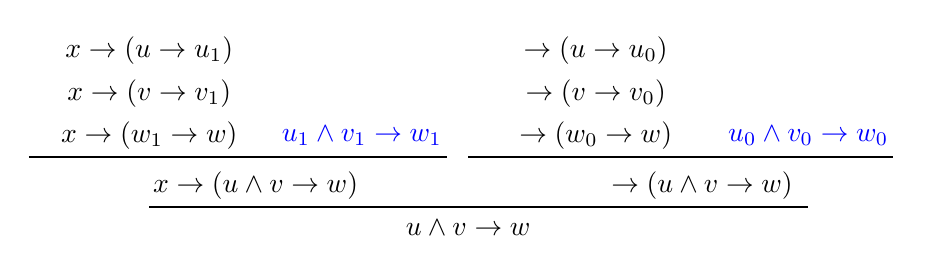
\begin{tikzpicture}[scale=0.9]

\node at (0,0) {$x \rightarrow (u \rightarrow u_1)$};
\node at (0,-0.6) {$x \rightarrow (v \rightarrow v_1)$};
\node at (0,-1.2) {$x \rightarrow (w_1 \rightarrow w)$};
\node at (3,-1.2) {\textcolor{blue}{$u_1 \land v_1 \rightarrow w_1$}};

\draw[thick] (-1.7,-1.5) -- (4.2,-1.5);

\node at (1.5, -1.9) {$ x \rightarrow (u \land v \rightarrow w)$};

\node at (6.3,0) {$\xnot \rightarrow (u \rightarrow u_0)$};
\node at (6.3,-0.6) {$\xnot \rightarrow (v \rightarrow v_0)$};
\node at (6.3,-1.2) {$\xnot \rightarrow (w_0 \rightarrow w)$};
\node at (9.3,-1.2) {\textcolor{blue}{$u_0 \land v_0 \rightarrow w_0$}};

\draw[thick] (4.5,-1.5) -- (10.5,-1.5);

\node at (7.8, -1.9) {$\xnot \rightarrow (u \land v \rightarrow w)$};

\draw[thick] (0,-2.2) -- (9.3,-2.2);


\node at (4.5, -2.5) {$u \land v \rightarrow w$};
\end{tikzpicture}
\end{center}
Can perform with 2 RUP steps


%% \!\!\!\!
%% {\bf Nuances}
%% \begin{itemize}
%% \item Many special cases when recursive arguments and results contain equivalences, 0s, and 1s.
%% \end{itemize}

}

\frame{
\frametitle{Quantification Operations}

{\bf Operation ${\sf EQuant}(f, X)$}
\begin{itemize}
%% \item Resulting function independent of variables in $X$
\item Abstract away details of satisfying (partial) solutions
\item Not logically required for SAT solver
\begin{itemize}
\item But, critical for obtaining good performance
\end{itemize}
\end{itemize}

\bigskip

{\bf Proof Generation}
\begin{itemize}
\item Do not attempt to follow recursive structure of algorithm
\item Instead, follow with separate implication proof generation
\begin{itemize}
\item ${\sf EQuant}(u, X) \rightarrow w$
\item Generate proof $u \rightarrow w$
\item Algorithm similar to proof-generating Apply operation
\end{itemize}
\end{itemize}


}

\frame{
\frametitle{Overall Proof Task}

{\bf Input Variables}

\vspace{20pt}

{\bf Input Clauses}
\begin{itemize}
\item Set of input clauses $C_I$ over the input variables
\end{itemize}

\vspace{20pt}

{\bf Completion}
\begin{itemize}
\item Generate Proof $C_I \vDash \bot$
\end{itemize}

}

\frame{

  \frametitle{Trusted BDDs (TBDD)}

\bigskip


{\bf Components}
\begin{itemize}
\item BDD with root node $t$
\item Proof step for unit clause $(t)$
\end{itemize}

\bigskip

{\bf Interpretation}
\begin{itemize}
\item $C_I \vDash t$
\item Any variable assignment that satisfies input clauses must yield $1$ for BDD with root $t$
\end{itemize}

} %% Frame

\frame{
  \frametitle{TBDD Example}

  \begin{minipage}[t]{\textwidth}
  \begin{minipage}{0.48\textwidth}
    \centering{
    \begin{tabular}{cl}
%      \toprule
      \makebox[0.5in][c]{$C_1$} & \makebox[1.0in][l]{$\anot \lor b$}  \\
      $C_2$ & $a \lor \cnot$  \\
      & \\
%      \bottomrule
    \end{tabular}
    } % centering
  \end{minipage}
  \begin{minipage}{0.48\textwidth}
    \centering{
    \begin{tabbing}
      $t_1 \assign {\it FromClause}(C_1)$ \\
      $t_2 \assign {\it FromClause}(C_2)$ \\
      \only<2->{$t_3 \assign {\it ApplyAnd}(t_1, t_2)$} \\
    \end{tabbing}
    } % centering
  \end{minipage}
  \end{minipage}

\centering{
\input{bdd-dd/tbdd}
} % centering


} % frame






\frame{
\frametitle{Structure of Overall Proof}

{\bf Input Variables}
\begin{itemize}
\item BDD variable for each input variable
\end{itemize}
\only<2->{
{\bf Input Clauses}
\begin{itemize}
\item For each input clause $C_i \in C_I$, generate BDD representation $t_i$
\item Generate {\em validation} proof $C_i \vDash t_i$
\begin{itemize}
\item Sequence of resolution steps based on linear structure of BDD
\end{itemize}
\item Initial set of TBDDs
\end{itemize}
}
\only<3->{
{\bf Combine Top-Level BDDs}
\begin{itemize}
\item Choose TBDDs $t_{i}$, $t_j$.  Use to generate TBDD $t_k$
\item $t_k \assign{} {\sf ApplyAnd}(t_i, t_j)$
\begin{itemize}
\item Combine proofs $C_I \vDash t_i$, $C_I \vDash t_j$ and $t_i \land t_j \rightarrow t_k$ to validate $C_I \vDash t_k$
\end{itemize}
\item $t_k \assign{} {\sf EQuant}(t_i, X)$
\begin{itemize}
\item Combine proofs $C_I \vDash t_i$ and $t_i \rightarrow t_k$ to validate $C_I \vDash t_k$
\end{itemize}
\end{itemize}
}
\only<4->{
{\bf Completion}
\begin{itemize}
\item When $t_k  = \bot$ have proof $C_I \vDash \bot$
\end{itemize}
}

}

\begin{frame}
  \frametitle{Comparing Proofs}

  {\bf Generated by CDCL Solver}
  \begin{itemize}
  \item Resolution
  \item Encode conflict clauses
    \begin{itemize}
    \item Increasingly strong constraints on set of satisfying solutions
    \end{itemize}
  \item Reach empty clause when detect there is no solution
  \end{itemize}

    \medskip

    {\bf Generated with BDD-Based Solver}
    \begin{itemize}
    \item Extended resolution
    \item Justify each recursive step of BDD algorithm
    \item Reach empty clause when reduce formula to BDD leaf $\bot$
    \end{itemize}

    \medskip

    {\bf Checking}
    \begin{itemize}
      \item Both checked with DRAT/LRAT checkers
    \end{itemize}

\end{frame}
  


\frame{
\frametitle{TBSAT (Trusted BDD Satisfiability solver)}


{\bf Implementation}
\begin{itemize}
\item TBUDDY: Modified version of BuDDy BDD package
  \begin{itemize}
    \item Lind-Nielsen, ca.~1998
  \end{itemize}
\item Support for TBDDs and proof generation
\item C/C++
\item \hcref{https://github.com/rebryant/tbuddy-artifact}  
\end{itemize}

\bigskip


}

\begin{frame}
\frametitle{Parity Benchmark Proof Complexity}

\centering{
\begin{tikzpicture}[scale = .80]
          \begin{axis}[mark options={scale=0.5},grid=both, grid style={black!10}, ymode=log, xmode=log, legend style={at={(0.95,0.35)}}, legend cell align={left},
                              x post scale=1.6,
                              xtick={10,100,1000,10000,100000}, xticklabels={$10$,$100$,$1{,}000$,$10{,}000$,$100{,}000$},xmin=10,xmax=100000,ymin=100,ymax=1000000000,
            %%                  title={Parity Benchmark Runtime}
            ]
       \input{data-formatted/chew-kissat-clauses}
       \input{data-formatted/chew-tbsat-direct-clauses}
       \input{data-formatted/chew-tbsat-bucket-clauses}
            \legend{
              \small \textsf{KISSAT},
              \small \textsf{TBSAT, Direct},
              \small \textsf{TBSAT, Bucket}
            }
          \end{axis}
\end{tikzpicture}
} % Centering

\begin{itemize}
\item Total number of proof steps
  \begin{itemize}\item Defining clauses + RUP clauses\end{itemize}
\item TBSAT with bucket elimination scales polynomially 
  \begin{itemize}
   \item  Checker time $\approx$ Solver time
  \end{itemize}
\end{itemize}

\end{frame}

\frame{
\frametitle{Integrating Parity Reasoning into Proof-Generating SAT Solver}

\begin{tikzpicture}[scale=0.3]
\draw[fill=structure] (1.0,1.0) rectangle (7.0,5.0);
\draw[fill=structure] (1.0,8.0) rectangle (7.0,12.0);
\draw[fill=white] (10.5,0.0) rectangle (21.5,13.5);
\draw[fill=structure] (12.0,1.0) rectangle (20.0,5.0);
\draw[fill=structure] (12.0,6.0) rectangle (20.0,10.0);
\draw (7.0,3.0) [-latex, line width=2pt] -- (12.0,3.0);
\draw (4.0,8.0) [-latex, line width=2pt] -- (4.0,5.0);
\draw (4.0,7.0) [-latex, line width=2pt] -- (12.0,7.0);
\draw (4.0,14.0) [-latex, line width=2pt] -- (4.0, 12.0);
\draw (0.0,14.0) [-latex, line width=2pt] -- (8.0,14.0) -- (8.0,9.0) -> (12.0,9.0);
%\draw (0.0,14.0) [line width=2pt] -- (8.0,14,0);
%\draw (8.0,14.0) [line width=2pt] -- (8.0,9.0);
%\draw (8.0,9.0) [-latex, line width=2pt] -- (12.0, 9.0);
\draw (21.5,6.0) [-latex, line width=2pt] -- (23.5,6.0);
\node [left] at (0.0,15.4) {Boolean};
\node [left] at (0.0,14.0) {Formula};
\node [left] at (0.0,12.6) {(CNF)};
\node [left] at (4.0,6.6) {Parity Formula};
\node [above] at (8.75,3.0) {Steps};
\node [right] at (23.5,6.8) {UNSAT};
\node [right] at (23.5,5.2) {Proof};
\node [white] at (4.0,10.8) {Parity};
\node [white] at (4.0,9.2) {Extractor};
\node [white] at (4.0,3.8) {Parity};
\node [white] at (4.0,2.2) {Solver};
\node [white] at (16.0,3.8) {Parity Step};
\node [white] at (16.0,2.2) {Validation};
\node [white] at (16.0,8.8) {CNF-Parity};
\node [white] at (16.0,7.2) {Validation};
\node at (16.0,12.5) {BDD-Based};
\node at (16.0,11.0) {Proof Generator};
\end{tikzpicture}

\begin{itemize}
\item Overall flow same as SAT solver
\item Parity solver does all of the reasoning
\item BDDs serve only as mechanism for generating clausal proof
\end{itemize}


} %% frame


\frame{
  \frametitle{Gaussian Elimination Over GF2}

  {\bf System of Equations $E = \{ \mathbf{e}_1, \mathbf{e}_2, \ldots, \mathbf{e}_m \}$}

  \begin{displaymath}
    \mathbf{e}_i: \;\;\; \sum_{j=1,n} a_{i,j} \cdot x_j =  b_i
  \end{displaymath}

\only<1>{
{\bf Assume}
  \begin{itemize}
  \item $a_{i,j}, x_j \in \{0, 1\}$
  \item \makebox[10mm][r]{$a+b$}\makebox[8mm][c]{$\equiv$}\makebox[10mm][l]{$a \oplus b$}
  \item \makebox[10mm][r]{$a\cdot b$}\makebox[8mm][c]{$\equiv$}\makebox[10mm][l]{$a \land b$}
  \end{itemize}

  {\bf Capability}
  \begin{itemize}
  \item Can determine if there are any solutions for $x_1, x_2, \ldots, x_n$
  \end{itemize}
}

\only<2>{
{\bf Elimination Step}
\begin{enumerate}
\item Choose pivot equation $\mathbf{e}_s$ and variable $x_{t}$ such that $a_{s,t} \not = 0$
\item For each $i \not = s$:
  \begin{eqnarray*}
    \mathbf{e}_{i} & \leftarrow & \left \{ \begin{array}{ll}
      \mathbf{e}_{i} & \;a_{i,t} = 0 \\
      \mathbf{e}_{s} + \mathbf{e}_{i}, & \;a_{i,t} \not = 0
      \end{array} \right .
  \end{eqnarray*}
\begin{itemize}
\item Guarantees $a_{i,t} = 0$ for all $i \not = s$
\end{itemize}
\item Remove $\mathbf{e}_s$ from $E$ and repeat until single equation left
\end{enumerate}
}
} % frame

\frame{
  \frametitle{Gaussian Elimination Results}
{\bf Possible Outcomes}
\begin{enumerate}
\item
 If encounter degenerate equation
  \begin{itemize}
    \item  Of form $0 = 1$
    \item Has no solution
  \end{itemize}

\item Otherwise, 
  \begin{itemize}
   \item Can perform back substitution to find solution
  \end{itemize}

\end{enumerate}

} %% frame

\frame{
  \frametitle{CNF to Parity Constraint Validation}
{\bf Clauses}
\begin{itemize}
\item Suppose clauses $C_{i_1}, C_{i_2}, \ldots, C_{i_k}$ encode parity constraint equation $\mathbf{e}$
\item Have validated BDD representations $t_{i_1}, t_{i_2}, \ldots, t_{i_k}$
\end{itemize}

{\bf Form conjunction}
  \begin{eqnarray*}
    s & = & \bigwedge_{1 \leq j \leq k} t_{i_j}
  \end{eqnarray*}
\begin{itemize}
\item Also yields proof $C_I \vDash s$
\end{itemize}

{\bf Represent Constraint}  
\begin{itemize}
\item Form BDD representation $t_j$ of $\mathbf{e}$
\end{itemize}

{\bf Validate}
\begin{itemize}    
\item Generate proof $s \rightarrow t_j$
\item Use to validate term $C_I \vDash t_j$
\end{itemize}

} %% frame

\frame{
  \frametitle{Parity Step Validation}

{\bf Assume}
\begin{itemize}
\item Have BDDs $t_{i}$ and $t_{j}$ representing equations $\mathbf{e}_i$ and $\mathbf{e}_j$
\item Satisfying $C_I \vDash t_{i}$ and $C_I \vDash t_{j}$
\end{itemize}

{\bf Compute}
\begin{itemize}
\item  $s  \assign {\it ApplyAnd}(t_i, t_j)$
  \begin{itemize}
  \item Gives proof $t_i \land t_j \rightarrow s$
  \end{itemize}
\item Generate BDD representation $t_k$ of equation $\mathbf{e}_k = \mathbf{e}_i + \mathbf{e}_j$
\end{itemize}

{\bf Validation}
\begin{itemize}
  \item Generate proof $s \rightarrow t_k$
  \item Combine with other proofs to validate $C_I \vDash t_k$
\end{itemize}


} %% frame

\begin{frame}
\frametitle{Parity Benchmark Runtime}

\centering{%
\begin{tikzpicture}[scale = .80]
          \begin{axis}[mark options={scale=0.5},grid=both, grid style={black!10}, ymode=log, ymin=0.01, ymax=600.0, xmode=log, legend style={at={(0.95,0.35)}}, legend cell align={left},
                              x post scale=1.6,
                              ytick={0.01,0.1, 1.0, 10.0, 100.0, 600.0}, yticklabels={$0.01$,$0.1$,$1.0$,$10.0$,$100.0$,$600.0$},
                              xtick={10,100,1000,10000,100000}, xticklabels={$10$,$100$,$1{,}000$,$10{,}000$,$100{,}000$},xmin=10,xmax=100000,
            %%                  title={Parity Benchmark Runtime}
            ]
       \input{data-formatted/chew-kissat-seconds}
       \input{data-formatted/chew-tbsat-direct-seconds}
       \input{data-formatted/chew-tbsat-bucket-seconds}
       \input{data-formatted/chew-tbsat-gauss-seconds}
            \legend{
              \small \textsf{KISSAT},
              \small \textsf{TBSAT, Direct},
              \small \textsf{TBSAT, Bucket},
              \small \textsf{TBSAT, Gauss}
            }
          \end{axis}
\end{tikzpicture}
}

\begin{itemize}
\item $n=100{,}000$ in 74 seconds
\item Upper limit: $n=699{,}051$
\begin{itemize}
  \item BuDDy limited to $2^{21}-1$ BDD variables
  \end{itemize}
\end{itemize}
\end{frame}


\begin{frame}
\frametitle{Parity Benchmark Proof Complexity}

\centering{
\begin{tikzpicture}[scale = .80]
          \begin{axis}[mark options={scale=0.5},grid=both, grid style={black!10}, ymode=log, xmode=log, legend style={at={(0.95,0.35)}}, legend cell align={left},
                              x post scale=1.6,
                              xtick={10,100,1000,10000,100000}, xticklabels={$10$,$100$,$1{,}000$,$10{,}000$,$100{,}000$},xmin=10,xmax=100000,ymin=100,ymax=1000000000,
            %%                  title={Parity Benchmark Runtime}
            ]
       \input{data-formatted/chew-kissat-clauses}
       \input{data-formatted/chew-tbsat-direct-clauses}
       \input{data-formatted/chew-tbsat-bucket-clauses}
       \input{data-formatted/chew-tbsat-gauss-clauses}
            \legend{
              \small \textsf{KISSAT},
              \small \textsf{TBSAT, Direct},
              \small \textsf{TBSAT, Bucket},
              \small \textsf{TBSAT, Gauss}
            }
          \end{axis}
\end{tikzpicture}
} % Centering

\begin{itemize}
\item Total number of proof steps
  \begin{itemize}\item Defining clauses + RUP clauses\end{itemize}
   \item  Checker time $\approx$ Solver time
\end{itemize}

\end{frame}

\frame{
  \frametitle{Final Thoughts on SAT Solvers}


  {\bf CDCL is the best overall approach}
    \begin{itemize}
      \item Readily generates resolution proofs
      \item But, very weak for parity and cardinality constraints
    \end{itemize}
  {\bf  BDDs provide complementary strengths}
    \begin{itemize}
    \item Can generate extended resolution proofs
    \item Very strong for parity constraints
    \item Some success with cardinality constraints
    \end{itemize}
  {\bf Future solvers should use combination of methods}
    \begin{itemize}
    \item With unified proof framework
    \item Clausal reasoning
    \item Constraint reasoning
    \item Boolean reasoning
    \end{itemize}

}

\frame{
  \frametitle{Final Thoughts on Checkable Proofs}

  {\bf Important capability}
  \begin{itemize}
    \item Vital to gain confidence in automated reasoning tools
    \item Benefits both tool developers and tool users
  \end{itemize}


  {\bf SAT community handled this especially well}
      \begin{itemize}
      \item Started with well-established logical framework (resolution)
      \item Developed efficient algorithms that integrated well with solvers (RUP)
      \item Included more general capabilities (extended resolution)
      \item Formulated file formats, tool chain
      \item Fostered deployment through competitions
      \end{itemize}
  
 {\bf More challenging for other domains}
      \begin{itemize}
      \item Beyond Boolean
      \end{itemize}

}


\frame{
  \frametitle{Some References}

{\bf BDDs}
\begin{itemize}
  \item R. E. Bryant, ``\cref{https://www.cs.cmu.edu/~bryant/pubdir/ieeetc86.pdf}{Graph-Based Algorithms for Boolean Function Manipulation},'' {\em IEEE Transactions on Computers}, 1986
  \item R. E. Bryant, ``\cref{https://www.cs.cmu.edu/~bryant/pubdir/hmc-bdd18.pdf}{Binary Decision Diagrams},'' {\em Handbook of Model Checking}, 2018
\end{itemize}

{\bf Proof Generation with BDDs}
\begin{itemize}
\item R. E. Bryant and M. J. H. Heule, ``\cref{https://www.cs.cmu.edu/~bryant/pubdir/tacas21.pdf}{Generating Extended Resolution Proofs with a BDD-Based SAT Solver},'' {\em TACAS}, 2021
\item R. E. Bryant, A. Biere, and M. J. H. Heule, ``\cref{https://www.cs.cmu.edu/~bryant/pubdir/tacas22-bbh.pdf}{Clausal Proofs from Pseudo-Boolean Reasoning},'' {\em TACAS}, 2022
\item R. E. Bryant, ``TBUDDY: A Proof-Generating BDD Package,'' {\em in submission}, 2022
\end{itemize}


}

\end{document}
